\chapter{Implementation}

VisuaLearn AI was implemented as a full-stack learning platform in which the browser interface, API server, database layer, AI-service calls, and generated learning resources are kept as separate parts of the system. The implementation follows the design described in the previous chapter and converts it into working modules for conversation, structured learning material, simulations, visual content, voice interaction, feedback, and persistence.

\section[Development Environment]{\textbf{Development Environment}}
The frontend was developed with React and Vite. React was used to build reusable interface components, while Vite provided the local development server and production build pipeline. Tailwind CSS was used for styling, spacing, and responsive behaviour. Framer Motion was included only for limited interface transitions where movement helped the user understand a state change.

The backend was developed with Node.js and Express.js. Express route modules expose the application features through API endpoints, while middleware handles authentication, validation, rate control, and error handling. Supabase provides user authentication, PostgreSQL storage, and file storage. The source code is divided into separate frontend and backend folders so that interface changes, API logic, and database access can be maintained independently.

\section[Frontend Implementation]{\textbf{Frontend Implementation}}
The frontend is organised around pages, reusable components, and custom hooks. The main pages include the home page, authentication pages, chat page, learning page, dashboard, and settings page. Shared interface components include the sidebar, message list, message bubble, learning workspace, voice overlay, simulation viewer, widget frame, persona card, and feedback controls.

The chat page acts as the learner's starting point. A submitted question is sent to the backend, and the response is streamed back into the conversation view. Tool choices such as quiz, flashcard, mind map, simulation, or visualisation are represented in the input area before submission so that the learner can see what has been selected and remove it if needed.

The learning page displays generated resources in separate sections instead of placing every resource in one long output. Explanations, examples, flashcards, quizzes, mind maps, simulations, and visualisations are shown only when the corresponding section is opened or when the selected mode requires it. This layout reduces crowding on smaller screens and keeps the learner focused on the current activity.

Custom hooks are used for stateful frontend tasks. Chat streaming, authentication state, learning-resource loading, simulation state, voice recording, feedback submission, progress tracking, and stored-resource retrieval are handled outside the display components. This keeps the rendering components smaller and makes the behaviour easier to test and update.

\section[Backend Implementation]{\textbf{Backend Implementation}}
The backend is structured into route modules, middleware, service functions, agents, database clients, and utility functions. Each feature has a clear entry point through the API layer. Separate route modules handle chat, learning content, simulation, visualisation, voice sessions, document resources, personas, user progress, and stored learning resources.

Authentication middleware verifies the user before protected routes are executed. Request validation checks the shape of incoming data before it reaches the service layer. Rate limiting protects expensive endpoints, especially those that can call external AI services. Error handling middleware returns controlled error responses and prevents internal details from being exposed to the client.

The chat and learning endpoints support streamed responses. Streaming is used because generated educational answers may take several seconds, and the learner should be able to start reading while the remaining content is still being produced. Each generated response is linked to a conversation record so that the learner can reopen previous sessions and continue from stored context.

\section[Learning Content Implementation]{\textbf{Learning Content Implementation}}
The learning-content module converts a user question into structured study material. The output is not limited to a single explanatory paragraph. Depending on the request and the selected tool, the backend can prepare conceptual explanations, worked examples, analogies, flashcards, quiz questions, mind-map nodes, and summary blocks.

\begin{itemize}[leftmargin=1.2cm]
	\item Conceptual explanations
	\item Examples and analogies
	\item Flashcards
	\item Quiz questions
	\item Mind map nodes
	\item Summary blocks
\end{itemize}

Generated resources are normalised before they are returned to the frontend. Normalisation gives the interface predictable fields for titles, content blocks, choices, answers, nodes, and metadata. This avoids forcing the frontend to parse free-form text for every resource type.

Resource generation is also lazy where possible. For example, flashcards or quiz questions can be generated when the learner opens that section rather than during the first answer. Stored resources are reused when available, which reduces repeated calls to the backend and keeps later visits to the same conversation faster.

\section[Adaptive Learning Implementation]{\textbf{Adaptive Learning Implementation}}
The adaptive layer records learner signals and uses them to select a response strategy. The context vector includes cognitive state, engagement level, topic status, performance trend, confidence, topic difficulty, previous failures, and response time. These values are collected or derived before the next response is generated.

The supported teaching strategies are:
\begin{enumerate}[leftmargin=1.2cm]
	\item Visual learning for concepts that need diagrams or widgets.
	\item Guided steps for procedures and algorithms.
	\item Quiz mode for checking understanding.
	\item Concise explanation for short clarification.
	\item Socratic questioning for guided reflection.
	\item Remediation for correcting misconceptions.
\end{enumerate}

After a strategy is selected, the backend adds the corresponding instruction to the generation request. The generated answer is then checked for basic structural compliance. For example, a quiz response should contain a question, and a guided-step response should contain an ordered explanation. Feedback such as quiz correctness, completion, and engagement is recorded so that later response selection can use evidence from previous interactions.

\begin{figure}[H]
\centering
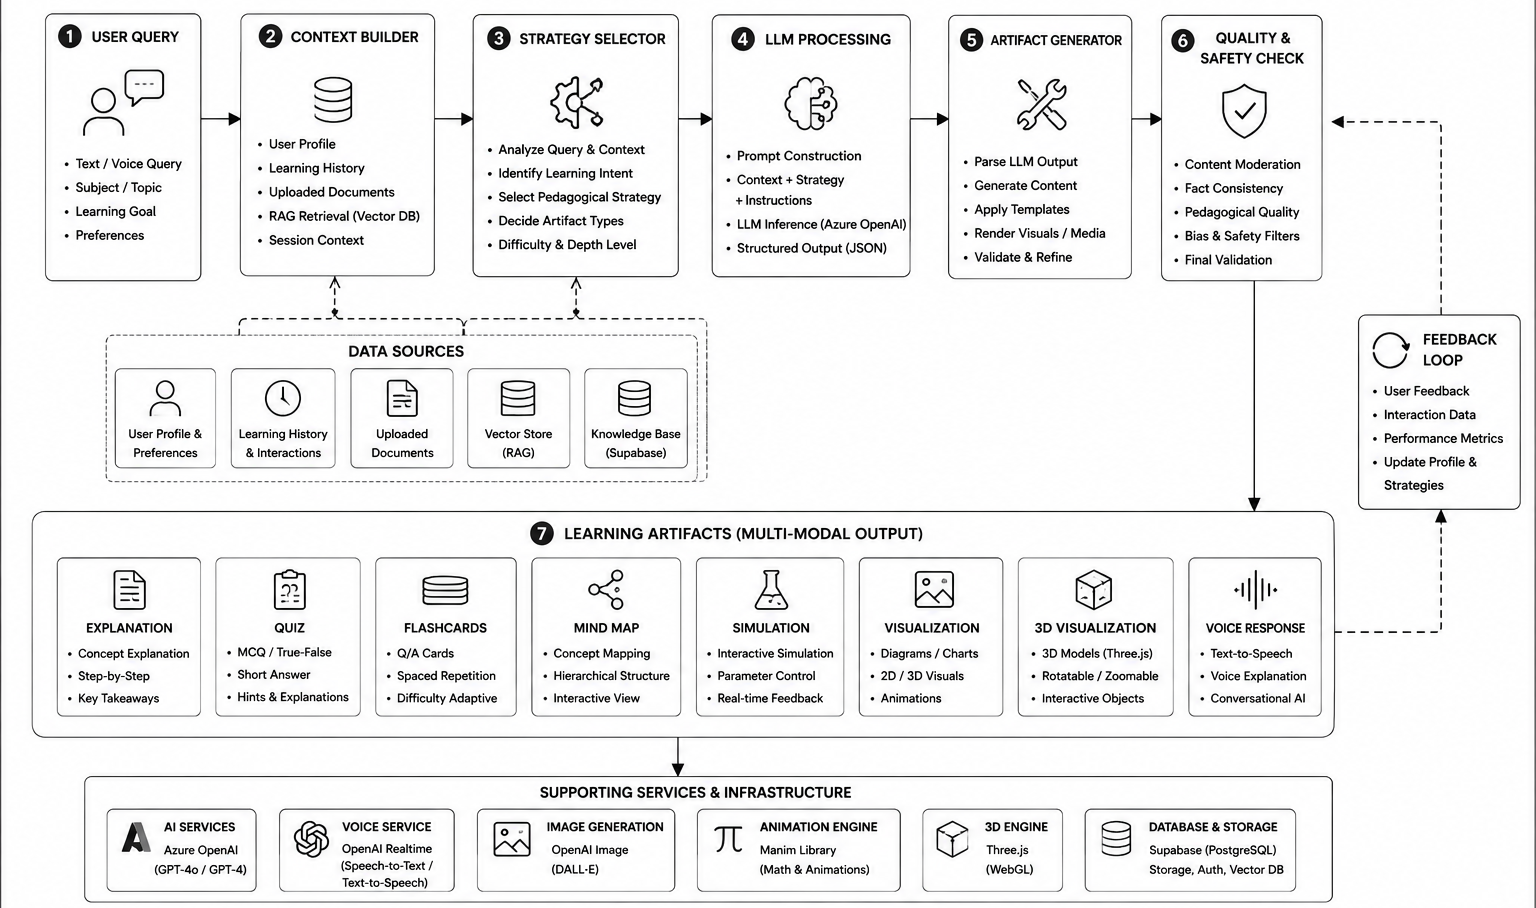
\includegraphics[width=0.92\textwidth]{Chapter4/some}
\caption{Adaptive strategy selection workflow}
\label{fig:adaptive-selection-strategy}
\end{figure}

\section[Simulation Implementation]{\textbf{Simulation Implementation}}
The simulation module first checks whether the requested topic can be represented as a sequence of observable states. Suitable topics include sorting algorithms, graph traversal, stacks, queues, heaps, linked lists, trees, state machines, grids, and timelines. When a topic is suitable, the backend prepares steps that describe how the state changes over time.

The frontend simulation viewer renders these steps with controls for play, pause, next, previous, and reset. The learner can inspect a single state or move through the process in order. In bubble sort, the viewer can show comparisons and swaps. In graph traversal, it can show the order in which nodes are visited. This stepwise display makes intermediate operations visible instead of presenting only the final answer.

\section[Visualization Implementation]{\textbf{Visualization Implementation}}
The visualisation module is used when a topic benefits from spatial, structural, or process-based representation. Before rendering, the system checks whether the generated visual content is safe and whether the device can support the required display. This prevents unsuitable visual output from affecting the rest of the application.

Generated visual widgets are displayed inside an isolated frame. The frame separates generated visual content from the main application interface. The content is validated and sanitised before display, and fallback messages are shown when rendering is not possible. This approach allows dynamic visual material to be used without giving generated content access to the main application state.

\section[Voice Interaction Implementation]{\textbf{Voice Interaction Implementation}}
The voice module allows a learner to ask questions through speech. The frontend records microphone input and connects it to a backend voice session. The backend associates the voice session with the learner context and the active conversation. Transcripts are written back into the chat flow so that spoken interactions remain part of the learning history.

Voice support is useful for short follow-up questions and revision sessions. It also improves access for learners who prefer speaking or who find typed interaction slower. The implementation keeps voice as an optional input path, so the normal text-based workflow remains available at all times.

\section[Persistence Implementation]{\textbf{Persistence Implementation}}
Persistence is implemented through Supabase. The database stores users, conversations, messages, learning resources, personas, feedback records, and adaptive decision records. Each generated learning resource is connected to a conversation. This allows the learner to reopen a previous session and access saved notes, flashcards, quizzes, mind maps, simulations, and visual resources.

The storage layer also reduces repeated generation. If a resource already exists for a conversation, the frontend can load it from storage instead of requesting a new generation. This improves response time and reduces unnecessary calls to external AI services.

\section[Deployment Architecture]{\textbf{Deployment Architecture}}
The deployment architecture separates the browser client, backend API, database services, storage, and external AI providers. The React client communicates with the Express backend through protected API routes. The backend performs authentication checks, request validation, learning orchestration, document retrieval, and AI-service calls. Supabase stores authenticated user data, conversations, generated learning resources, feedback records, and uploaded document metadata.

\begin{figure}[H]
\centering
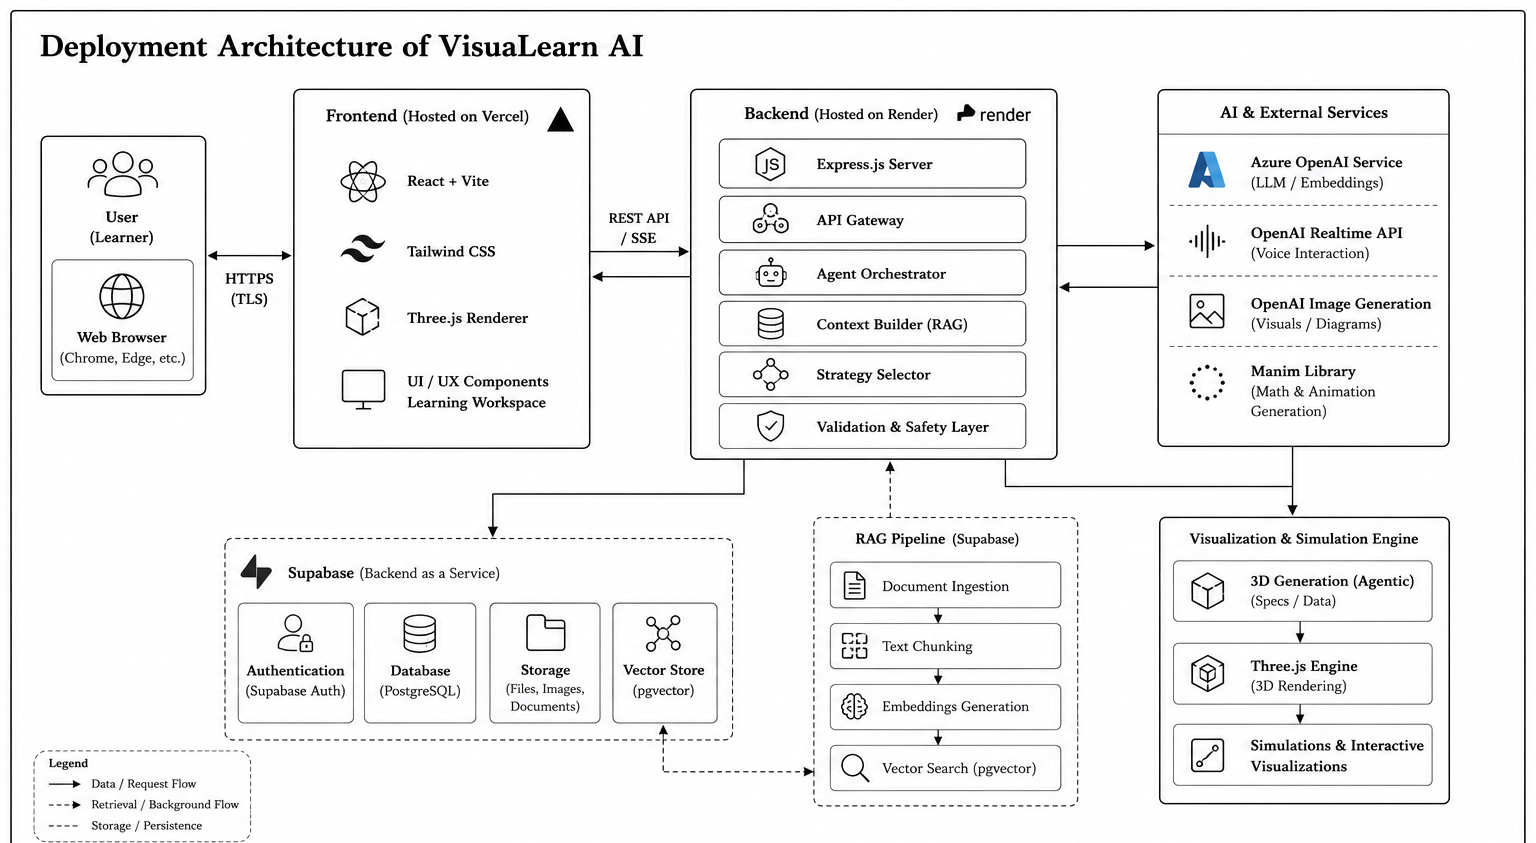
\includegraphics[width=0.92\textwidth]{Chapter4/dep}
\caption{Deployment architecture of VisuaLearn}
\label{fig:deployment-architecture}
\end{figure}

Provider keys and service credentials are kept on the server side. The browser sends requests to the backend rather than calling AI providers directly. This arrangement reduces credential exposure and allows backend routes, database storage, frontend hosting, and AI-service usage to be scaled or monitored separately.

\section[Security and Reliability Implementation]{\textbf{Security and Reliability Implementation}}
The implementation includes security and reliability measures at several points in the request flow:
\begin{itemize}[leftmargin=1.2cm]
	\item Protected routes for authenticated users.
	\item Request validation for malformed inputs.
	\item Rate limiting for controlled usage.
	\item Isolated rendering for generated visual artifacts.
	\item Fallback responses when a module fails.
	\item Structured logging for debugging and monitoring.
	\item Caching for repeated or expensive operations.
\end{itemize}

These measures are intended to keep failures local to the affected feature. For example, if a generated widget cannot be displayed, the chat and stored learning resources should still remain usable. Similarly, if a cached resource is available, the learner can continue studying even when a new generation request is delayed.

\section[Implementation Summary]{\textbf{Implementation Summary}}
The implementation delivers the main workflow required by VisuaLearn AI. A learner can ask questions, receive structured explanations, open revision resources, run simulations, view visual material, use voice input, submit feedback, and return to stored sessions. The modular structure keeps the main features separate while allowing them to operate together through shared conversation records, learner context, and stored resources.
